\input{header}

\AtBeginSubsection[]
{
	\begin{frame}<beamer>
		\frametitle{Outline}
		\tableofcontents[current,currentsubsection]
	\end{frame}
}

\begin{document}



\begin{frame}[allowframebreaks] 
\frametitle{Pushdown automata}
\begin{itemize}
\item Context-free languages are more general than regular
  languages
\item For regular languages, by definition, there are automata to
  recognize them
\item What are machines to recognize CFL?
\item Pushdown automata (PDA)

\item [] It's more powerful by having a \alert{stack}
\item DFA (or NFA):
\begin{center}
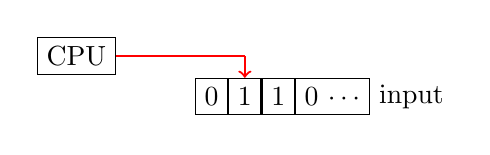
\begin{tikzpicture}[ampersand replacement=\&]
\matrix 
{
  \node[draw](0) {CPU}; \& [1cm] \& \node(1){}; \&\&\& \\
  \& \node[draw]{0}; \& \node[draw](a){1}; \& \node[draw]{1}; \& \node[draw]{0 $\cdots$};  \& \node{input};\\
};
\draw [-,red,thick] (0) -- (1.center) ;
\draw [->,red,thick] (1.center) -- (a) ;
\end{tikzpicture}
\end{center}
\item Pushdown automata:
\begin{center}
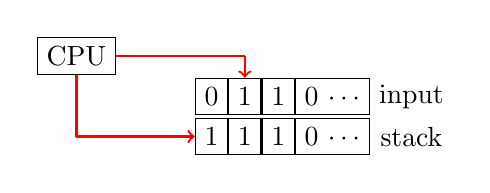
\begin{tikzpicture}[ampersand replacement=\&]
\matrix 
{
  \node[draw](0) {CPU}; \& [1cm]  \& \node(1){} ; \&\&\& \\
  \& \node[draw]{0}; \& \node[draw](a){1}; \& \node[draw]{1}; \& \node[draw]{0 $\cdots$};  \& \node{input};\\
\node(c){}; \& \node[draw](b){1}; \& \node[draw]{1}; \& \node[draw]{1}; \& \node[draw]{0 $\cdots$}; \&  \node{stack}; \\
};

\draw [-,red,thick] (0) -- (1.center) ;
\draw [->,red,thick] (1.center) -- (a) ;
\draw [-,red,thick] (0) -- (c.center) ;
\draw [->,red,thick] (c.center) -- (b) ;
\end{tikzpicture}
\end{center}

\item What is a stack?

\item [] We know they are like plates in a cafeteria

\item [] An important property: \alert{last in first out}
\item Let's see how stack can help to recognize
  \begin{equation*}
\{0^n 1^n\mid n \geq 0\}
\end{equation*}
\item[] If 0 is read, 0 is pushed to stack
\item If 1 is read, 0 is popped up
\item By checking (0, 1) pairs, we know if the input is
  $0^n 1^n$
\end{itemize}
\end{frame}

\begin{frame}[allowframebreaks] \frametitle{Example 2.14}
  \begin{itemize}
  \item Consider the following language
    \begin{equation*}
    \{0^n 1^n\mid n \geq 0\}
  \end{equation*}

\begin{center}
\begin{tikzpicture}
\node[state,initial,accepting] (q_1) {$q_1$};
\node[state] (q_2) [right of=q_1] {$q_2$};
\node[state] (q_3) [below of=q_2] {$q_{3}$};
\node[state,accepting] (q_4) [left of=q_3] {$q_{4}$};      
  \path 
  (q_1) edge[above]  node {$\epsilon, \epsilon \rightarrow \$ $} (q_2)
  (q_2) edge[loop right]  node {$0,\epsilon \rightarrow 0$} (q_2)
  (q_2) edge[right]  node {$1, 0 \rightarrow \epsilon$} (q_3)
  (q_3) edge[loop right]  node {$1, 0 \rightarrow \epsilon$} (q_3)  
  (q_3) edge[below] node {$\epsilon, \$ \rightarrow \epsilon$} (q_4);
  \end{tikzpicture}
\end{center}
\item \$: a special symbol to indicate the initial state of stack

  
\item How it works:
  \item [] $q_2 \rightarrow q_2$, put 0 into stack

  \item [] $q_2 \rightarrow q_3$ and $q_3 \rightarrow q_3$, read 1 and  pop 0 up

  \begin{equation*}
    0011
  \end{equation*}

the same as
  \begin{equation*}
    \epsilon 0011 \epsilon
  \end{equation*}
\item Steps:
  \begin{equation*}
    \begin{split}
& q_1, \emptyset, \epsilon\\
& q_2, \{\$\}, 0 \\
& q_2, \{0,\$\}, 0\\
& q_2, \{0,0,\$\}, 1\\
& q_3, \{0,\$\}, 1\\
& q_3, \{\$\}, \epsilon\\
& q_4, \{\}
\end{split}
\end{equation*}
$\{\}$: contents of the stack

\item We see that \$ can be used to check
  if the stack is empty

\item Consider 00011
\item [] Steps:
  \begin{equation*}
    \begin{split}
& q_1, \epsilon, \{\$\} \\
& \vdots \\
& q_2, 0, \{0, 0,0,\$\}\\
& q_3, 1, \{0, 0, \$\}\\
& q_3, 1, \{0, \$\}
\end{split}
\end{equation*}
Cannot reach $q_4$ $\Rightarrow$ rejected  
\end{itemize}\end{frame} \begin{frame}[allowframebreaks] \frametitle{Formal definition of pushdown automata}
  \begin{itemize}  
\item $(Q,\Sigma, \Gamma, \delta, q_0, F)$

\item [] $Q, \Sigma, \Gamma, F$: finite sets
\begin{enumerate}
\item $Q$: states
\item $\Sigma$: alphabet
\item $\Gamma$: stack alphabet
\item $\delta$:
  \begin{equation*}
  Q \times 
\Sigma_{\epsilon} \times \Gamma_{\epsilon}
\rightarrow P(Q\times \Gamma_\epsilon)
\end{equation*}
\item $q_0 \in Q$: start state
\item $F \subset Q$: set of accept states
\end{enumerate}
\item We rely on
  \begin{center}
  state, input, \alert{top of stack}
\end{center}
to decide the move
\begin{equation*}
q_1 \stackrel{a,b \rightarrow c}{\longrightarrow}
q_2
\end{equation*}
From $q_1$, read $a$, and replace top of stack
$b$ with $c$
\end{itemize}\end{frame} \begin{frame}[allowframebreaks] \frametitle{Formal definition of example 2.14}
  \begin{itemize}
  \item The language is
    \begin{equation*}
    \{0^n 1^n\mid n \geq 0\}
  \end{equation*}
\item $M_1 = (Q,\Sigma, \Gamma, \delta, 
q_1, F)$
\begin{equation*}
  \begin{split}
& Q=\{q_1, q_2, q_3, q_4\} \\
& \Sigma=\{0,1\} \\
& \Gamma=\{0,\$\} \\
& F=\{q_1, q_4\}
\end{split}
\end{equation*}

{
\setlength{\tabcolsep}{3pt}  
\begin{tabular}{@{}lccc|ccc|ccc@{}}

&
\multicolumn{3}{c|}{0} &
\multicolumn{3}{c|}{1} &
\multicolumn{3}{c}{$\epsilon$}\\ \hline
& 0 & \$ & $\epsilon$ 
& 0 & \$ & $\epsilon$ 
& 0 & \$ & $\epsilon$ \\ \hline
$q_1$ &&&&&&&&& $\{(q_2,\$)\}$\\
$q_2$ &&&$\{(q_2,0)\}$&$\{(q_3,\epsilon)\}$&&&&& \\
$q_3$ &&&&$\{(q_3,\epsilon)\}$&&&&$\{(q_4,\epsilon)\}$& \\
$q_4$ &&&&&&&&& \\ 
\end{tabular}
}

\item In the definition of $\delta$ we have
  $\Sigma_\epsilon \times \Gamma_\epsilon$
\item [] Thus 9 columns in the table

\end{itemize}\end{frame} \begin{frame}[allowframebreaks] \frametitle{Example 2.16}

  \begin{equation*}
  \{a^i b^j c^k
\mid i=j \mbox{ or } i = k\}
\end{equation*}
  \begin{itemize}
\item Idea: put $a^i$ into stack

\item [] But should we check $b$ or $c$ ?

\item Need \alert{nondeterminism}
\item Pushdown automata may be nondeterministic
\item Recall $\delta$ was defined as
    \begin{equation*}
  Q \times 
\Sigma_{\epsilon} \times \Gamma_{\epsilon}
\rightarrow P(Q\times \Gamma_\epsilon)
\end{equation*}
We see the power set $P(Q\times \Gamma_\epsilon)$ 
\item Fig 2.17
\end{itemize}

\scalebox{0.9}{
\begin{tikzpicture}
\node[state,initial] (q_1) {$q_1$};
\node[state] (q_2) [right of=q_1] {$q_2$};
\node[state] (q_3) [above right of=q_2] {$q_{3}$};
\node[state,accepting] (q_4) [right of=q_3] {$q_{4}$};
\node[state] (q_5) [below right of=q_2] {$q_{5}$};
\node[state] (q_6) [right of=q_5] {$q_{6}$};      
\node[state,accepting] (q_7) [right of=q_6] {$q_{7}$};      

\path 
(q_1) edge[above]  node {$\epsilon, \epsilon \rightarrow \$ $} (q_2)
(q_2) edge[loop above]  node {$a,\epsilon \rightarrow a$} (q_2)
(q_2) edge[right]  node {$\epsilon, \epsilon \rightarrow \epsilon$} (q_3)
(q_2) edge[right]  node {$\epsilon, \epsilon \rightarrow \epsilon$} (q_5)
(q_3) edge[loop above]  node {$b, a \rightarrow \epsilon$} (q_3)
(q_3) edge[above]  node {$\epsilon, \$ \rightarrow \epsilon$} (q_4)
(q_4) edge[loop above]  node {$c, \epsilon \rightarrow \epsilon$} (q_4)
(q_5) edge[loop below]  node {$b, \epsilon \rightarrow \epsilon$} (q_5)
(q_5) edge[below]  node {$\epsilon, \epsilon \rightarrow \epsilon$} (q_6)
(q_6) edge[loop below]  node {$c, a \rightarrow \epsilon$} (q_6)
(q_6) edge[below] node {$\epsilon, \$ \rightarrow \epsilon$} (q_7);
  \end{tikzpicture}
}

\begin{itemize}
\item nondeterminism: $q_2 \rightarrow q_3$
or $q_2 \rightarrow q_5$

and others ($q_5 \rightarrow q_5
$ or $q_5 \rightarrow q_6$)

one for $b^i$ and one for $c^i$

\item Exercise: $a^2bc^2$ (a tree)

  
\end{itemize}\end{frame}

\begin{frame}[allowframebreaks]
  \frametitle{Running a PDA}
  \begin{itemize}
  \item Input $a^2bc^2$
  \item The way is similar to how we run an NFA
\end{itemize}
  
  \begin{center}
\scalebox{0.9}{    
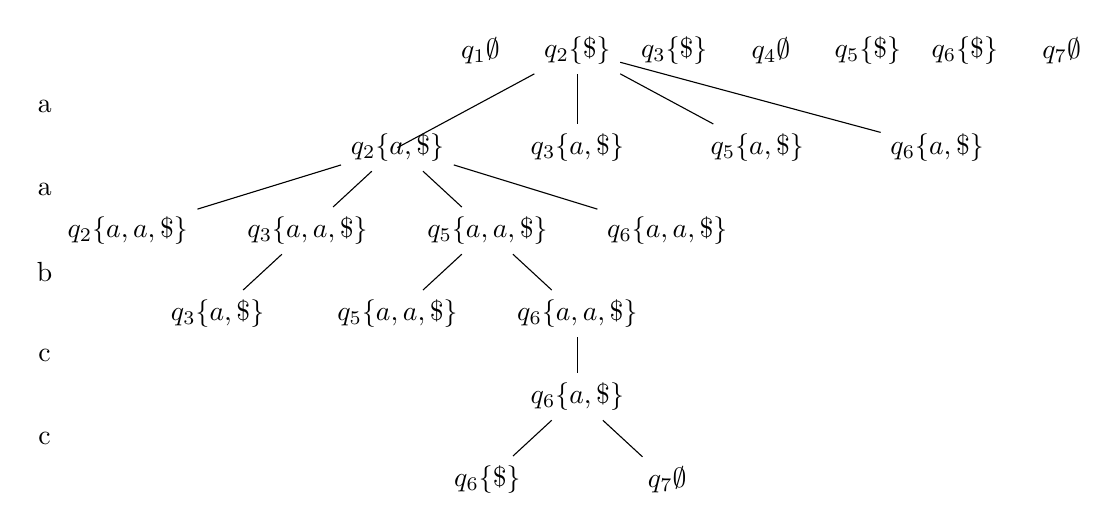
\begin{tikzpicture} [level distance=25pt,sibling distance=65pt]% grow=right
\node  {$q_1\emptyset$}
child [grow=right, level distance=35pt] { node  { $q_2\{\$\}$ } edge from parent[draw=none]
  [grow=down]
  child [grow=right] { [level distance=35pt] node  {$q_3\{\$\}$} edge from parent[draw=none]
    child [grow=right] {node  {$q_4\emptyset$} edge from parent[draw=none]
      child [grow=right] {node  {$q_5\{\$\}$} edge from parent[draw=none]
        child [grow=right] {node  {$q_6\{\$\}$} edge from parent[draw=none]
          child [grow=right] {node  {$q_7\emptyset$} edge from parent[draw=none]
          }
        }
      }
    }
  }
  child { [level distance=30pt] node  {$q_2\{a,\$\}$}
    child {node  {$q_2\{a,a,\$\}$}
      child [grow=left] {node (3) {} edge from parent[draw=none]
        child [grow=up] {node (2) {} edge from parent[draw=none]
          child [grow=up] {node (1) {} edge from parent[draw=none]
          }
        }
        child [grow=down] {node (4) {} edge from parent[draw=none]
          child [grow=down] {node (5) {} edge from parent[draw=none]
            child [grow=down] {node (6) {} edge from parent[draw=none]
            }
          }
        }
      }
    }
    child {node  {$q_3\{a,a,\$\}$}
      child {node  {$q_3\{a,\$\}$}
      }
      child {edge from parent[draw=none]}      
    }
    child {node  {$q_5\{a,a,\$\}$}
      child {node  {$q_5\{a,a,\$\}$}}
      child {node  {$q_6\{a,a,\$\}$}
        child {node  {$q_6\{a,\$\}$}
          child {node  {$q_6\{\$\}$}}
          child {node  {$q_7\emptyset$}}
        }
      }
    }
    child {node  {$q_6\{a,a,\$\}$}}
  }    
  child  {node {$q_3\{a,\$\}$}}      
  child  {node {$q_5\{a,\$\}$}}
  child  {node {$q_6\{a,\$\}$}}
};
\path (1) -- (2) node [midway] {a};
\path (2) -- (3) node [midway] {a};
\path (3) -- (4) node [midway] {b};
\path (4) -- (5) node [midway] {c};
\path (5) -- (6) node [midway] {c};
\end{tikzpicture}
}
\end{center}
\end{frame}

\begin{frame}[allowframebreaks] \frametitle{Example 2.18}
  \begin{itemize}
\item $\{ww^R\mid w \in \{0,1\}^*\}$

\item [] $w^R$: reverse
\item Approach:

\item [] symbols pushed to stack

\item [] nondeterministically guess middle is reached


\item fig 2.19

\begin{center}
\begin{tikzpicture}
\node[state,initial,accepting] (q_1) {$q_1$};
\node[state] (q_2) [right of=q_1] {$q_2$};
\node[state] (q_3) [below of=q_2] {$q_{3}$};
\node[state,accepting] (q_4) [left of=q_3] {$q_{4}$};      
  \path 
  (q_1) edge[above]  node {$\epsilon, \epsilon \rightarrow \$ $} (q_2)
  (q_2) edge[loop right]  node {
    \begin{tabular}{l}
      $0,\epsilon \rightarrow 0$\\
      $1,\epsilon \rightarrow 0$
    \end{tabular}
} (q_2)
  (q_2) edge[right]  node {$\epsilon \rightarrow \epsilon$} (q_3)
  (q_3) edge[loop right]  node {
    \begin{tabular}{l}
      $0, 0 \rightarrow \epsilon$
      \\
      $1, 1 \rightarrow \epsilon$
    \end{tabular}
} (q_3)  
  (q_3) edge[below] node {$\epsilon, \$ \rightarrow \epsilon$} (q_4);
  \end{tikzpicture}
\end{center}

  
\end{itemize}\end{frame} \begin{frame}[allowframebreaks] \frametitle{Equivalence with context-free grammars}
  \begin{itemize}  
\item Language context free
$\Leftrightarrow$ recognized by pushdown automata

\item Recall that by definition a language is context-free if
  it is constructed by some CFG
\item One direction is easier, while the other is harder
\item As usual, we do the easier one first
  
\end{itemize}\end{frame} \begin{frame}[allowframebreaks] \frametitle{CFL $\rightarrow$ PDA}
    \begin{itemize}
    \item Given a CFG, we find a PDA to simulate this grammar
      
\item Two keys:

\item [] stack 

\item [] nondeterminism: different substitutions

  
\item We do the proof by an example
\item Suppose we are given the following
  CFG
  \begin{equation*}
    \begin{split}
      & S \rightarrow aTb \mid b\\
      & T \rightarrow Ta \mid \epsilon
    \end{split}
  \end{equation*}

\item Idea: for rule substitution, push right-hand side to stack

\item [] For example, $aTb$ is pushed to stack in a reversed way

  \item
  A PDA can be as follows

\begin{tikzpicture}
\node[state,initial] (q_1) {$q_s$};
\node[state] (q_2) [below of=q_1,yshift=1.2cm] {};
\node[state] (q_3) [below of=q_2,yshift=1.2cm] {$q_{\text{loop}}$};
\node[state] (q_4) [above right of=q_3, yshift=-0.5cm, xshift=0.5cm] {};
\node[state] (q_6) [right of=q_4, yshift=1.8cm] {};
\node[state] (q_5) [below right of=q_3, yshift=0.5cm, xshift=2.5cm] {};
\node[state] (q_7) [below of=q_3,yshift=1.2cm,accepting] {$q_a$};
  \path 
  (q_1) edge[left]  node {$\epsilon, \epsilon \rightarrow \$ $} (q_2)
  (q_2) edge[left]  node {$\epsilon, \epsilon \rightarrow S $} (q_3)
  (q_3) edge[left]  node {$\epsilon, \$ \rightarrow \epsilon $} (q_7)    
  (q_3) edge[loop left]  node [xshift=-0.5cm] {
    \begin{tabular}{l}
      $\epsilon,S \rightarrow b$\\
      $\epsilon, T \rightarrow \epsilon$\\
      $a, a \rightarrow \epsilon$\\
      $b, b \rightarrow \epsilon$
    \end{tabular}
  } (q_3)
  (q_3) edge[right]  node {$\epsilon, S \rightarrow b$} (q_4)
  (q_4) edge[right]  node {$\epsilon, \epsilon \rightarrow T$} (q_6)
  (q_6) edge[bend right, above]  node {$\epsilon, \epsilon \rightarrow a$} (q_3)
  (q_3) edge[below, bend left]  node {$\epsilon, T \rightarrow a$} (q_5)
  (q_5) edge[below, bend left]  node {$\epsilon, \epsilon \rightarrow T$} (q_3)  
;
  \end{tikzpicture}

% \item Fig 2.22

% inermediate string: 01A1A0

% substitute A by ??

% check if finally it matches \$

\item Consider an example sequence $aaaab$
% Draw a tree process $aaaa$
% Before the first $a$, we will see $\infty$
% possibilities. Can handle this situation
% by confine the stack length to be smaller
% than the input length
\end{itemize}

\begin{eqnarray*}
&& q_{\text{start}} \stackrel{\epsilon}{\rightarrow}
q_{\text{loop}}, \{S,\$\} 
\stackrel{\epsilon}{\rightarrow} q_1, \{b,\$\}
\stackrel{\epsilon}{\rightarrow} q_2, \{T,b,\$\} \\
&& \stackrel{\epsilon}{\rightarrow} q_{\text{loop}}, \{a,T,b,\$\} 
\stackrel{a}{\rightarrow}
 q_{\text{loop}}, \{T,b,\$\} \\
&& \stackrel{\epsilon}{\rightarrow} q_{3}, \{a, b,\$\} 
\stackrel{\epsilon}{\rightarrow} q_{\text{loop}}, \{T,a,b,\$\}\\
&& \stackrel{\epsilon}{\rightarrow} q_3, \{a,a,b,\$\}
\stackrel{\epsilon}{\rightarrow} q_{\text{loop}}, \{T,a,a,b,\$\}\\
&& \stackrel{\epsilon}{\rightarrow} q_3, \{a,a,a,b,\$\}
\stackrel{\epsilon}{\rightarrow} q_{\text{loop}}, \{T,a,a,a,b,\$\}\\
&& \stackrel{\epsilon}{\rightarrow} q_{\text{loop}}, \{a,a,a,b,\$\}
\stackrel{a}{\rightarrow} q_{\text{loop}}, \{a,a,b,\$\}\\
&& \stackrel{a}{\rightarrow} q_{\text{loop}},\{a,b,\$\}
\stackrel{a}{\rightarrow} q_{\text{loop}}, \{b,\$\}\\
&& \stackrel{b}{\rightarrow} q_{\text{loop}}, \{\$\}
\stackrel{\epsilon}{\rightarrow} q_{accept}
\end{eqnarray*}

\end{frame}

\end{document}
